\documentclass[11pt,a4paper]{article}
\usepackage[utf8]{inputenc}
\usepackage[T1]{fontenc}
\usepackage{lmodern}
\usepackage[a4paper,margin=1in]{geometry}
\usepackage{amsmath,amssymb}
\usepackage{booktabs,array,graphicx,float,xcolor,url,xurl,caption}
\usepackage[colorlinks=true,linkcolor=blue,citecolor=blue,urlcolor=blue]{hyperref}
\usepackage[authoryear,round]{natbib}
\graphicspath{{../../results/figures/}}
% AUTO-GENERATED by scripts/09_make_numbers.py. Do not edit.
\newcommand{\GateOnePass}{18}
\newcommand{\GateOneFail}{0}
\newcommand{\PolicyTotal}{25}
\newcommand{\PolicyViable}{20}
\newcommand{\PolicyDropped}{5}
\newcommand{\SlowestSettleDay}{53}
\newcommand{\ViableMinCalmFill}{0.99}
\newcommand{\FluidK}{1.07}
\newcommand{\FluidRsq}{0.95}
\newcommand{\FluidN}{63}
\newcommand{\MildUnmetLo}{1.1}
\newcommand{\MildUnmetHi}{11.1}
\newcommand{\MildLossShareLo}{82}
\newcommand{\LiveCells}{17}
\newcommand{\DecidableMedian}{0.86}
\newcommand{\RandomRegretAboveDelta}{17}
\newcommand{\MddFiveSeeds}{1.8}
\newcommand{\MddThirtySeeds}{0.7}
\newcommand{\PilotSeeds}{5}
\newcommand{\PairsPerCell}{190}
\newcommand{\DeltaFill}{0.5}
\newcommand{\DeltaUnmet}{1.5}
\newcommand{\RunLength}{400}
\newcommand{\DisruptStart}{100}
   % auto-generated by scripts/09_make_numbers.py; never typed by hand

% Draft markers. Every unfinished part is visibly marked so nothing unfinished is mistaken for finished.
\newcommand{\todo}[1]{\textcolor{red}{[TODO: #1]}}
\newcommand{\pending}[1]{\textcolor{orange}{[PENDING DATA: #1]}}

\title{Can We Trust the Fast Copy? A Decision-Regret Validation of Machine-Learning Surrogates of Supply-Chain Simulators Under Disruption}
\author{Draft --- author block to be completed}
\date{Working draft, built \today}

\begin{document}
\maketitle

\begin{abstract}
\todo{Write last. One sentence each: the problem (surrogates are adopted on average error, not decision quality); what we did (timed disruptions, decision regret, decidable-pair rank flips with multiplicity control, conformal coverage under shift); the headline finding; what it implies.}
\end{abstract}

\section{Introduction}
\todo{Motivation (adoption--validation gap), the gap in the literature, contributions. Draft from \texttt{docs/proposal/proposal.tex} Sections 2--3 once the results exist, so the framing follows the findings rather than preceding them.}

\section{Related Work}
\todo{Port the landscape table and nearest-neighbour discussion from the proposal; re-verify every citation (several 2026 items were preprints).}

\section{Methods}\label{sec:methods}

\subsection{Study design in one paragraph}
We ask whether a fast machine-learning copy (``surrogate'') of a supply-chain simulator can be trusted to \emph{choose} between operating policies once conditions move beyond the disruptions it was trained on. Surrogates are trained only on mild, short disruptions and evaluated on harder and longer ones. The quantity of interest is \emph{decision regret}: the extra demand lost by acting on the surrogate's recommended policy instead of the simulator's best policy. Prediction error is reported alongside, because the two can disagree. Two simulators are used: an open platform with a disclosed modified fork (Simulator~B, \citealp{zhang2026isomorph}) and our own discrete-event simulator (Simulator~A, \pending{not yet built; Section~\ref{sec:simA} to be written when it exists}).

\subsection{Simulator B and the three disclosed modifications}\label{sec:simB}
Simulator~B is the ISOMORPH multi-echelon network simulator \citep{zhang2026isomorph}. We use a fork pinned at a fixed commit (\texttt{third\_party/ISOMORPH\_Hmod}) with three single-purpose changes, each a no-op at the released defaults and each verified as such against the released baseline before any experiment (\texttt{scripts/00\_patch\_verification.py}): (i) the duration of its random global shocks is scaled to the requested horizon, because at short horizons the released generator compounds into near-permanent disruption; (ii) capacity scaling acts on the continuous container-volume field after last-mile self-calibration, instead of an integer container count; (iii) a scheduled per-day capacity factor, applied on days $[t_0, t_0+D)$ and exactly 1 otherwise, produces timed, bounded disruptions. All runs use the proactive shipping rule that the released baseline uses (pipeline multiplier 7 by default), and the simulator's random global shocks are switched off in every run reported here, so that differences between runs are caused only by the factor varied. A white-box test confirms the capacity schedule: the factor equals the requested value exactly on the disrupted days and 1.0 on every other day, on every edge, and a zero-length disruption changes nothing (\GateOnePass{} integrity checks passed, \GateOneFail{} failed; Appendix~\ref{sec:app-valid}).

\subsection{Random numbers and pairing}
The simulator is deterministic given its seed (identical output on repeat). Customer demand is identical across policies and with or without a disruption for the same seed, so policy comparisons are paired on demand (common random numbers). Lead-time draws are \emph{not} paired across policies: they use a separate random stream that is consumed only when a node reorders. We therefore use paired tests on demand-matched runs and state this limitation.

\subsection{Disruption design: timed events indexed by overload}\label{sec:severity}
A disruption cuts every transport edge's capacity to a fraction $c$ of nominal for $D$ days starting at day $t_0=\DisruptStart$, then restores it. The last-mile tier of Simulator~B carries about $1.29\times$ nominal demand, so cuts down to $c\approx0.775$ are absorbed and lose nothing. We therefore index severity by \emph{overload},
\begin{equation}
\nu = \max\bigl(0,\; 1 - 1.29\,c\bigr),
\end{equation}
the share of demand the network cannot carry during the event. A scan over capacity level $\times$ duration (Appendix~\ref{sec:app-valid}) shows that recovery time follows $\mathrm{TTR}\approx k\,D\,\nu/0.29$ with $k=\FluidK$ ($R^2=\FluidRsq$, $n=\FluidN$ uncensored runs), i.e.\ the system behaves like a fluid queue that must drain the backlog accumulated during the event. Durations are 14, 30 and 90 days. Severity bands are Mild $0<\nu\le0.15$, Moderate $0.15$--$0.35$, Severe $0.35$--$0.55$, Extreme $0.55$--$0.68$. Surrogates are trained on Mild events of 14 and 30 days only; all other cells are test cells. A calm-only training arm and a wider training band ($\nu\le0.25$) are run as sensitivity analyses. \emph{Why timed events:} permanent capacity cuts below the stability boundary make backlog grow without bound, so no recovery or steady state exists to compare policies on (Appendix~\ref{sec:app-valid}).

\subsection{Warm-up and run length}
Every run has one fixed length $L=\RunLength$ days, identical for training and test data, so that the evaluation window is not confounded with the distribution shift. The calm regime settles by day 100 for the pilot warm-up study; across the \PolicyViable{} viable policies the slowest settles by day \SlowestSettleDay{} (noise-aware criterion), so the disruption starts after a 100-day warm-up. With the longest event ending on day 190, $L=\RunLength$ leaves 210 days for recovery; only the most extreme 90-day corner is right-censored at this length (Appendix~\ref{sec:app-valid}).

\subsection{Policies}
A policy is a pair (safety-stock scale $\in\{0.25,0.5,0.75,1,1.5\}$, pipeline multiplier $\in\{3,5,7,10,14\}$). Of the \PolicyTotal{} pairs, \PolicyDropped{} lose demand even in calm weather (calm fill rate below \ViableMinCalmFill) and are removed, leaving \PolicyViable{} viable policies and $\PairsPerCell$ policy pairs.

\subsection{Outcome metrics}
Outcomes are computed over the post-warm-up window $[t_0, L)$. The primary metric is \emph{unmet demand} in days of demand, because fill rate is a cliff metric that floors at zero in severe cells and stops discriminating. Secondary metrics are the resilience-triangle area \citep{bruneau2003}, peak backlog, and time-to-recovery, which is right-censored when recovery does not occur within $L$ \citep{henry2012}; recovery means seven consecutive days within 2 percentage points of the run's own pre-disruption baseline.

\subsection{Decidable policy pairs, multiplicity, and the practical margin}\label{sec:decidable}
A policy pair is \emph{decidable} in a cell when the paired mean difference exceeds a practical margin $\delta$ \emph{and} is significant after Benjamini--Hochberg false-discovery-rate control at $q=0.10$ \citep{benjamini1995} over all pairs in that cell. $\delta=\DeltaFill$ percentage points of fill rate, equivalent to \DeltaUnmet{} days of unmet demand at $L=\RunLength$. Rank flips between simulator and surrogate are counted only among decidable pairs, and a placebo run (simulator against an independent simulator replicate) gives the noise floor of the flip rate. \todo{Placebo and planted-flip dry runs not yet executed; fill in the results when they are.}

\subsection{Surrogate battery, conformal coverage, and shift protocols}
\todo{Port from the proposal once the battery is fixed: four families with nested cross-validation on training regimes only; split-conformal intervals with and without covariate-shift weighting \citep{tibshirani2019}; protocols P1 (severity/duration extrapolation) on both simulators, P2--P4 on Simulator~A only (B supports only timed capacity cuts).}

\subsection{Simulator A}\label{sec:simA}
\pending{Simulator A is not built. Its capacity margin will be set generously (2--3$\times$ nominal demand) following the stability-boundary finding on B; its warm-up pilot, cost coefficients and $\delta$ justification are written here when it exists.}

\subsection{Pre-specified rules and what was decided after looking at data}\label{sec:prereg}
To keep the analysis honest, every design choice that was made \emph{after} seeing pilot data is listed. (1) Severity was re-indexed from capacity fraction to overload $\nu$ after the first scan showed that the originally planned Mild band lost no demand. (2) Run length was raised from 300 to 400 days after the same scan showed that at 300 days every extreme 90-day cell was censored. (3) Five policies were dropped for failing in calm weather. (4) Cells in which fewer than 30\% of policy pairs are decidable are reported but excluded from the headline flip tables (rule fixed before any test data). Pilot seeds (2025--2029) are never reused for training, calibration, test or placebo data; those use disjoint seed ranges fixed in \texttt{src/scmval/design.py}.

\section{Results}
\pending{Training data, surrogate fits, regret, rank-flip tables, coverage. Nothing in this section may be written before the design is locked and the test data exist.}

\section{Discussion and Limitations}
\todo{Write after results. Known limitations already: Simulator~B lead times are unpaired across policies; B supports only timed capacity cuts; B's last-mile tier has thin margin so $\nu>0$ is needed for any effect; findings on two simulators are not findings on real supply chains.}

\section{Reproducibility}
All code, seeds, configurations and the pinned simulator fork are in a public repository (\url{https://github.com/nil0y-dey/scm-surrogate-validation}). Every number in this draft is generated from files in \texttt{results/reports/} by \texttt{scripts/09\_make\_numbers.py}. Runs are idempotent and checkpointed, so any session can resume.

\appendix
\section{Validation of Simulator B before data collection}\label{sec:app-valid}
\paragraph{Integrity.} Determinism, prefix identity (a disrupted and an undisrupted run with the same seed are identical before the disruption starts), demand pairing across policies, and the exact capacity schedule: \GateOnePass{} checks passed, \GateOneFail{} failed.
\paragraph{Warm-up and policy viability.} Figure~\ref{fig:warmup} shows the calm warm-up; Figure~\ref{fig:gate3} shows each policy's calm behaviour. \PolicyViable{} of \PolicyTotal{} policies are viable; the slowest settles by day \SlowestSettleDay{}.
\paragraph{What each severity does.} Figure~\ref{fig:gate4} shows unmet demand and recovery across overload and duration, and the fluid-queue fit ($k=\FluidK$, $R^2=\FluidRsq$).
\paragraph{Pilot policy power (not a result).} In a pilot of 5 seeds per cell, Mild training events lose between \MildUnmetLo{} and \MildUnmetHi{} days of demand on average (at least \MildLossShareLo\% of runs lose some). Over the \LiveCells{} cells with real loss, the median share of decidable policy pairs is \DecidableMedian{}, random policy advice costs more than $\delta$ in \RandomRegretAboveDelta{} of them, and the minimum detectable difference falls from \MddFiveSeeds{} days at 5 seeds to \MddThirtySeeds{} days at 30 seeds (Figure~\ref{fig:gate56}).

\begin{figure}[H]\centering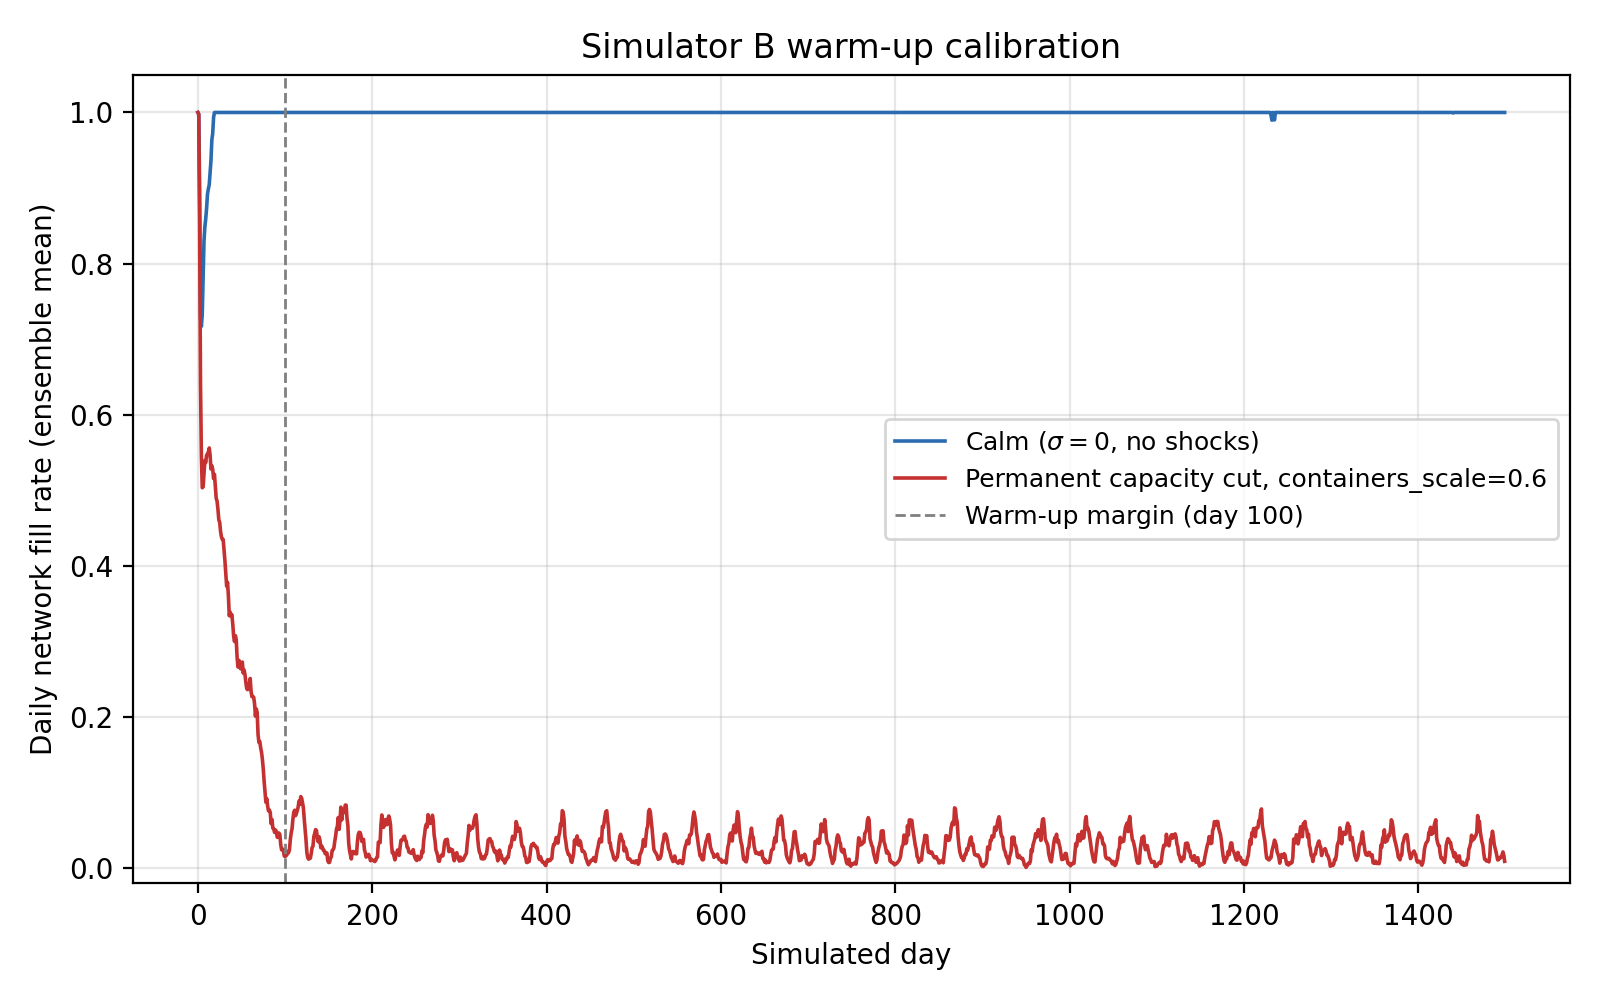
\includegraphics[width=0.7\textwidth]{warmup_figure.png}\caption{Calm warm-up of Simulator~B (5-seed ensemble mean).}\label{fig:warmup}\end{figure}
\begin{figure}[H]\centering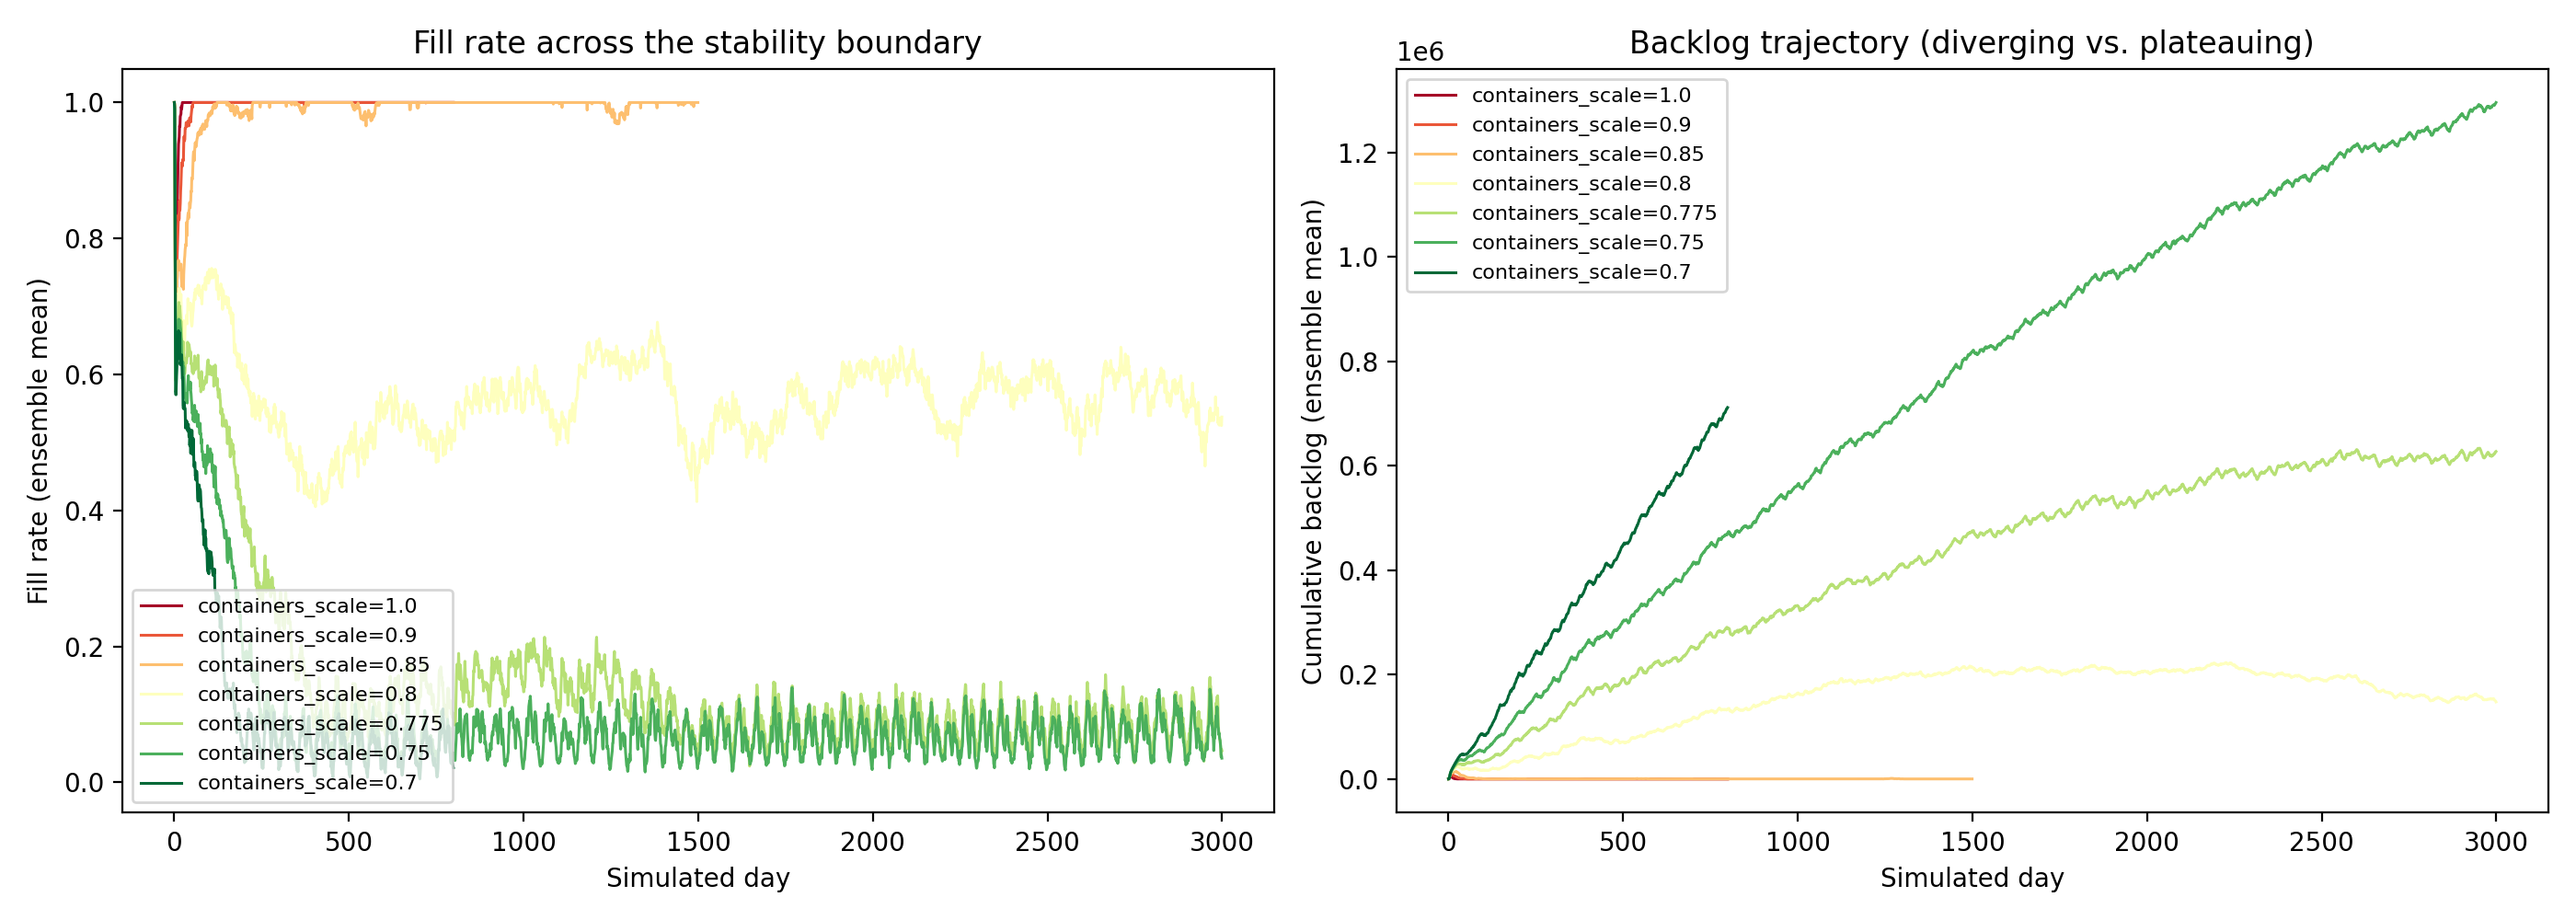
\includegraphics[width=0.9\textwidth]{stability_boundary_figure.png}\caption{Permanent capacity cuts: below the stability boundary backlog grows without bound.}\label{fig:stab}\end{figure}
\begin{figure}[H]\centering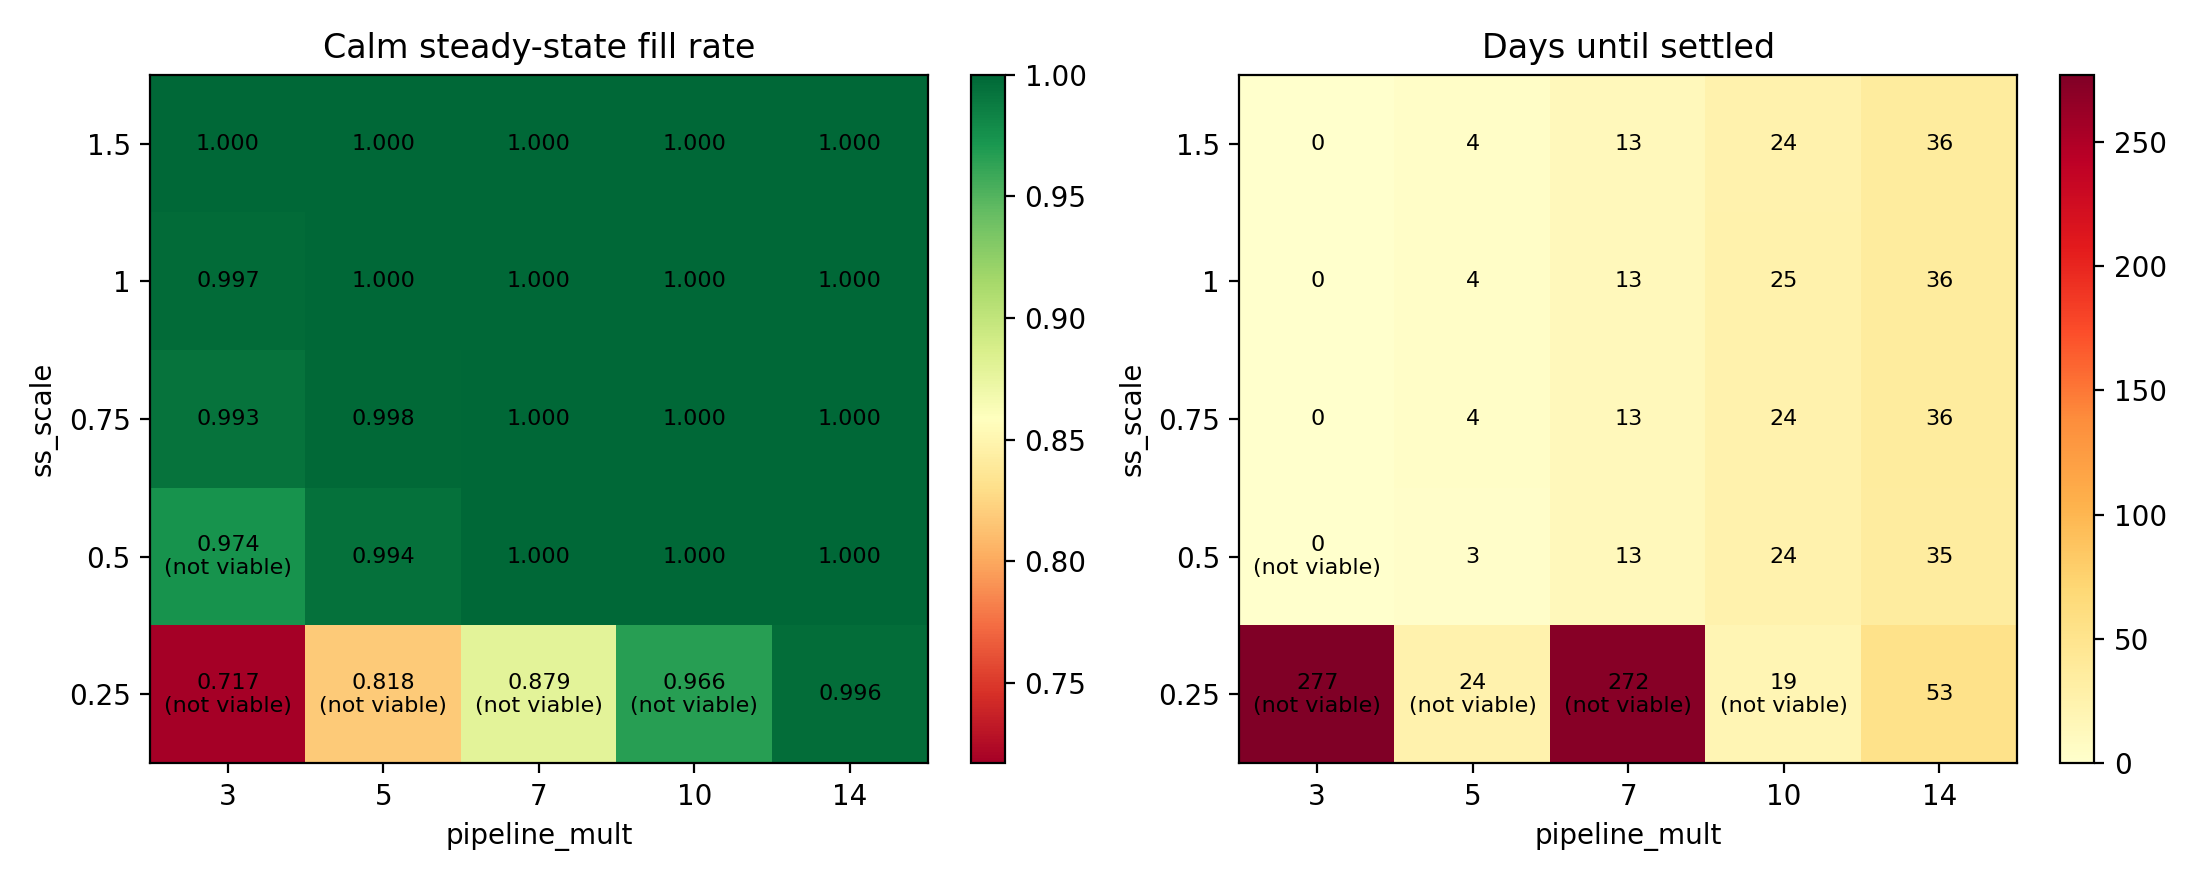
\includegraphics[width=0.9\textwidth]{gate3_policy_grid.png}\caption{Calm-weather behaviour of the 25 policies.}\label{fig:gate3}\end{figure}
\begin{figure}[H]\centering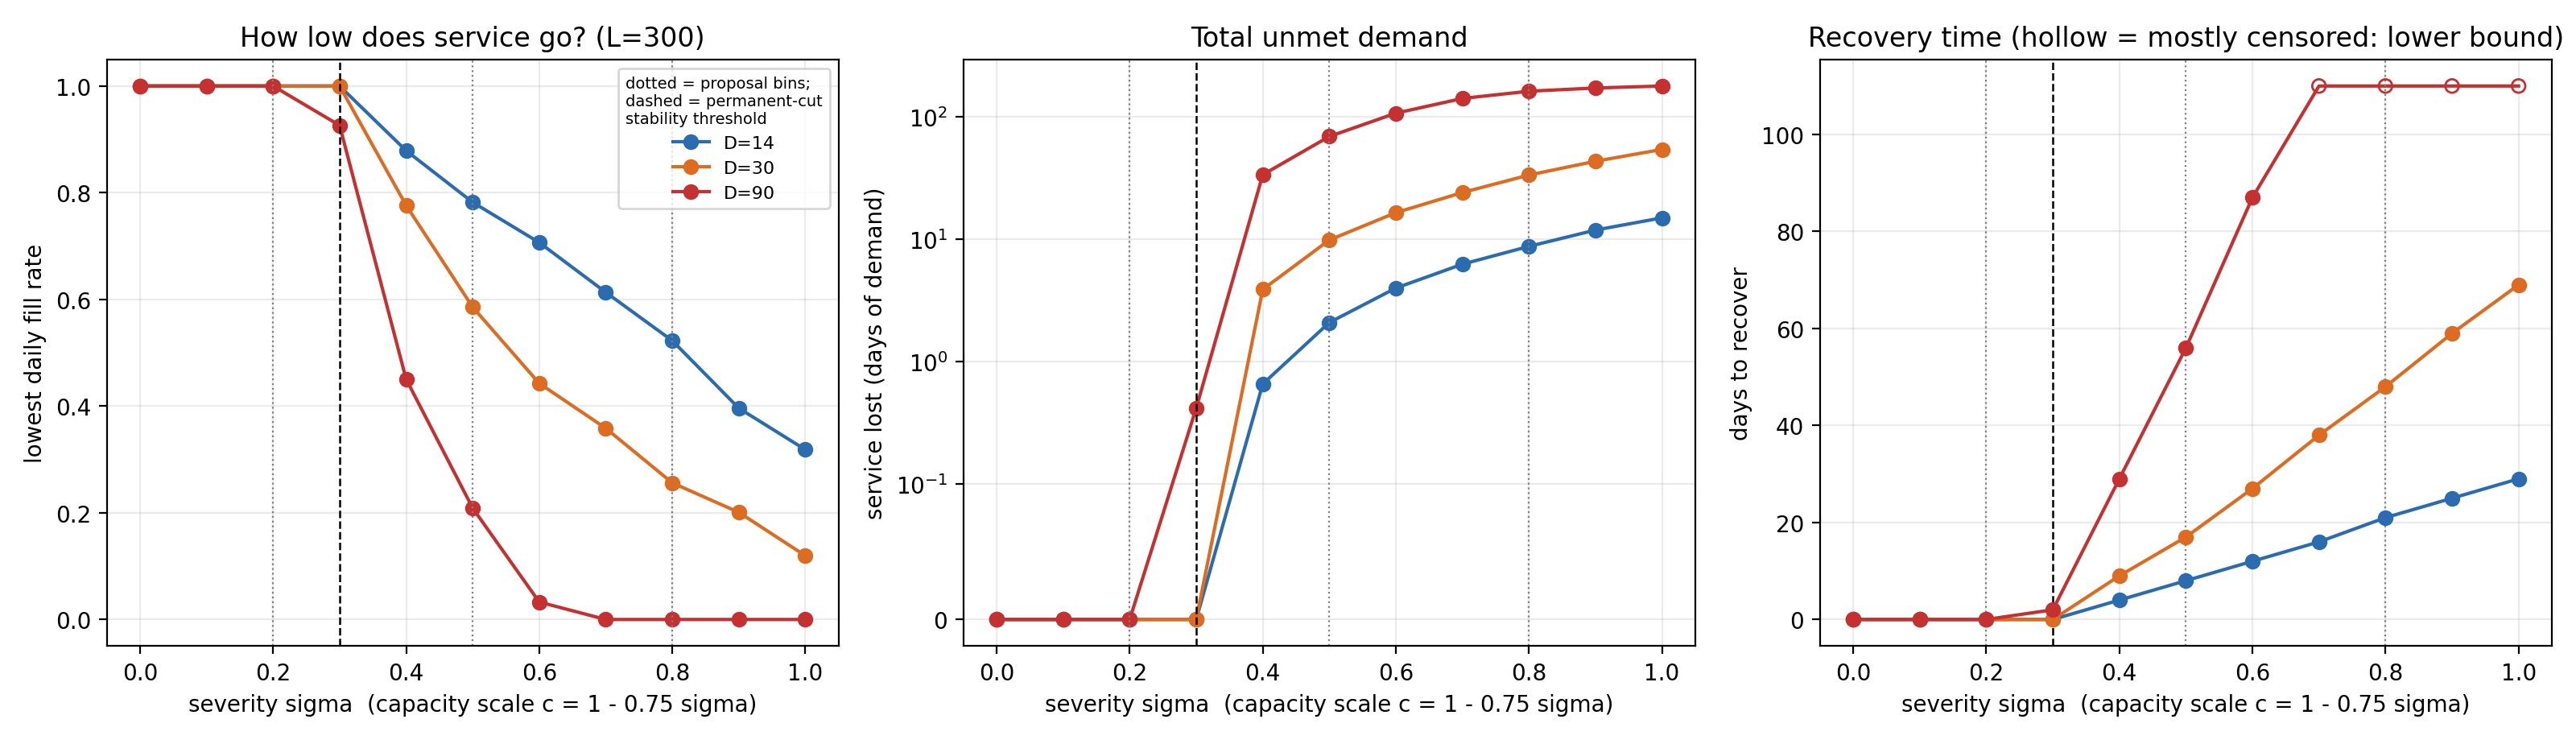
\includegraphics[width=0.9\textwidth]{gate4_mapping.png}\caption{Severity mapping scan.}\label{fig:gate4}\end{figure}
\begin{figure}[H]\centering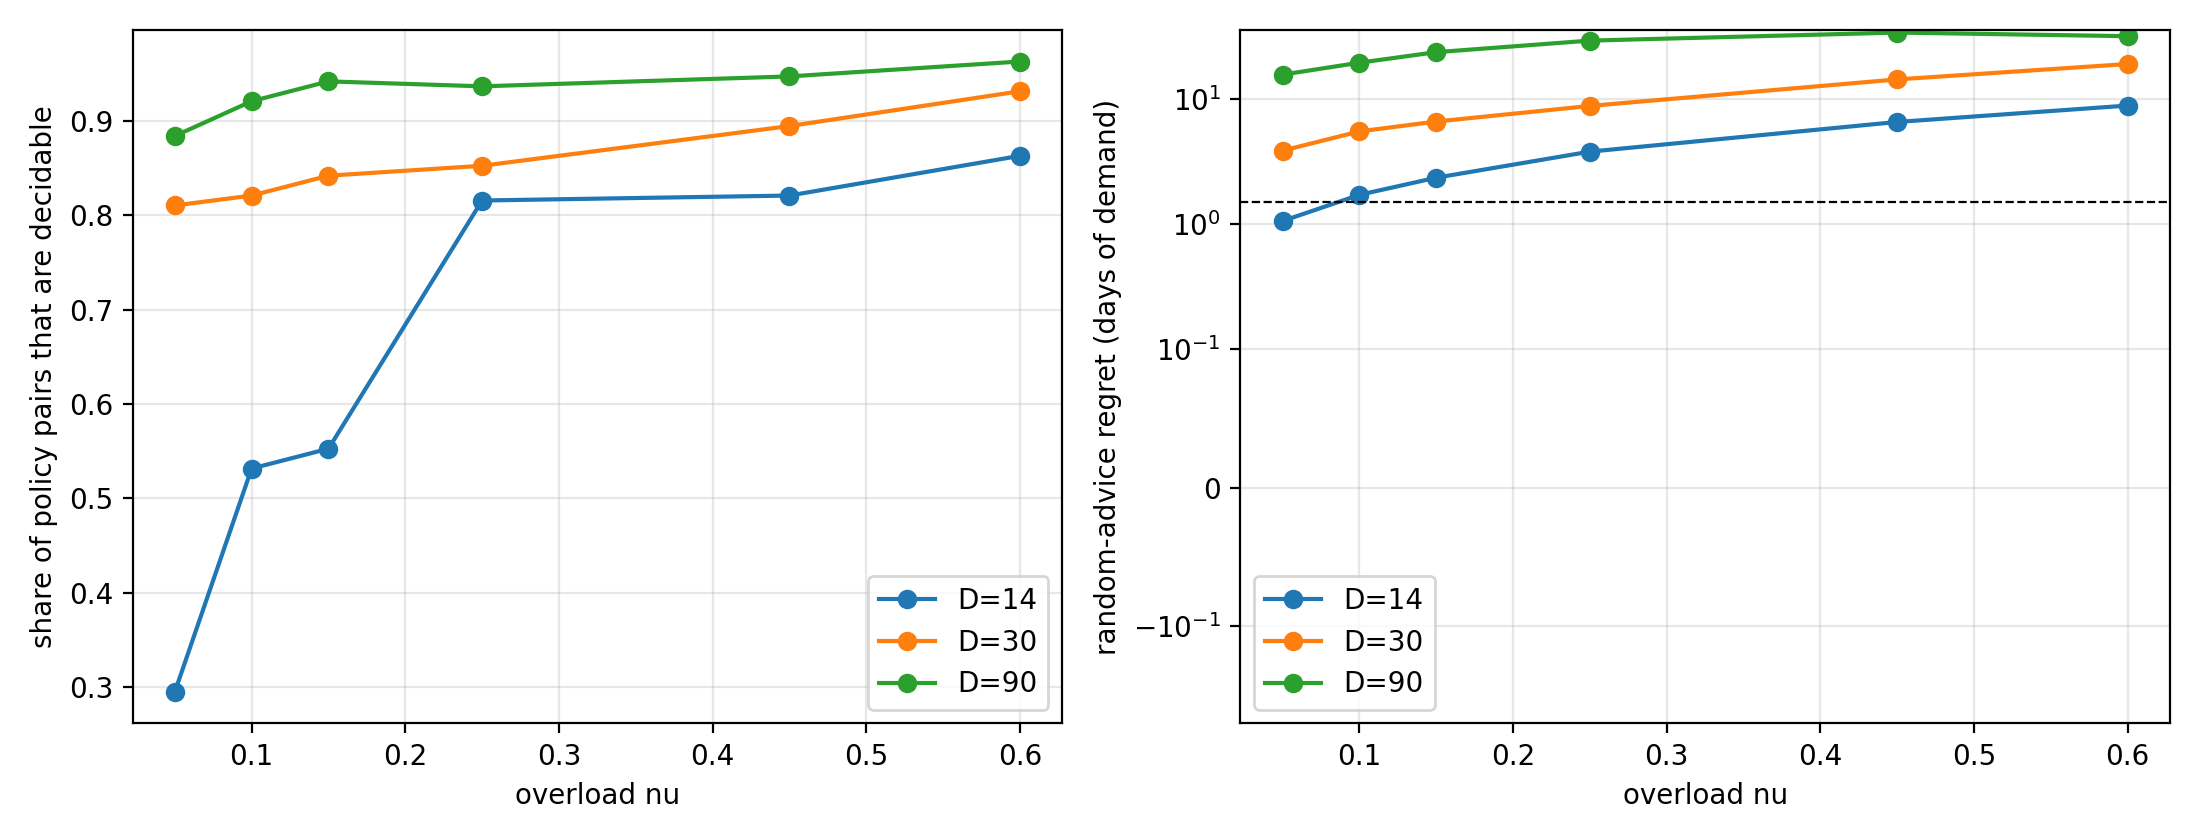
\includegraphics[width=0.9\textwidth]{gate56_power.png}\caption{Pilot policy power by overload and duration.}\label{fig:gate56}\end{figure}

\bibliographystyle{plainnat}
\begin{thebibliography}{99}
\bibitem[Benjamini and Hochberg(1995)]{benjamini1995} Benjamini, Y., \& Hochberg, Y. (1995). Controlling the false discovery rate: a practical and powerful approach to multiple testing. \textit{Journal of the Royal Statistical Society: Series B}, 57(1), 289--300.

\bibitem[Bruneau et al.(2003)]{bruneau2003} Bruneau, M., Chang, S.E., Eguchi, R.T., Lee, G.C., O'Rourke, T.D., Reinhorn, A.M., Shinozuka, M., Tierney, K., Wallace, W.A., \& von Winterfeldt, D. (2003). A framework to quantitatively assess and enhance the seismic resilience of communities. \textit{Earthquake Spectra}, 19(4), 733--752.

\bibitem[Henry and Ramirez-Marquez(2012)]{henry2012} Henry, D., \& Ramirez-Marquez, J.E. (2012). Generic metrics and quantitative approaches for system resilience as a function of time. \textit{Reliability Engineering and System Safety}, 99, 114--122.

\bibitem[Tibshirani et al.(2019)]{tibshirani2019} Tibshirani, R.J., Barber, R.F., Cand\`es, E., \& Ramdas, A. (2019). Conformal prediction under covariate shift. \textit{Advances in Neural Information Processing Systems (NeurIPS)}.

\bibitem[Zhang et al.(2026)]{zhang2026isomorph} Zhang, Z., Gu, H., Zhang, B.J., Elenius, D., Tyrrell, M., et al. (2026). ISOMORPH: a supply chain digital twin for simulation, dataset generation, and forecasting benchmarks. \textit{arXiv preprint}.

\end{thebibliography}
\end{document}
